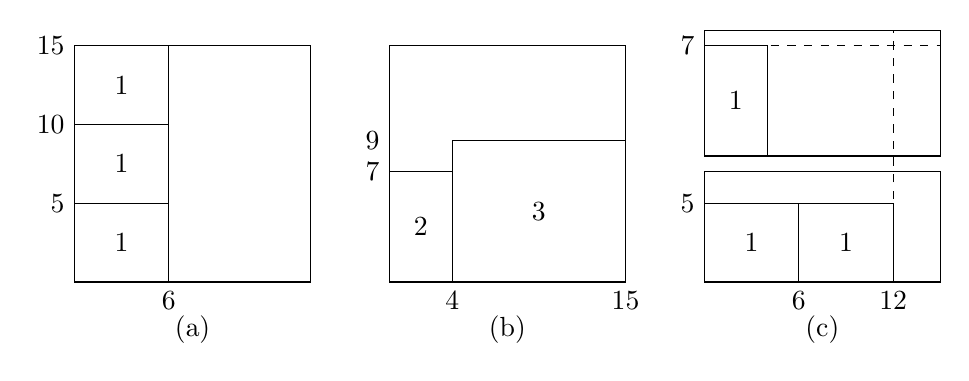
\begin{tikzpicture}[scale=0.20]
\begin{scope}[shift={(0, 0)}]
\draw [draw=black]   (0, 0) rectangle ++(15, 15);
\draw [draw=black]   (0, 0) rectangle     ++(6, 5) node [midway] {1};
\draw [draw=black]   (0, 5) rectangle     ++(6, 5) node [midway] {1};
\draw [draw=black] (0, 10) rectangle     ++(6, 5) node [midway] {1};
\node [left]  at (0, 5) {5};
\node [left]  at (0, 10) {10};
\node [left]  at (0, 15) {15};
\node [below]  at (6, 0) {6};
\node [below] at (7.5, -1.5) {(a)};
\end{scope}
\begin{scope}[shift={(20, 0)}]
\draw [draw=black]   (0, 0) rectangle ++(15, 15);
\draw [draw=black]   (0, 0) rectangle     ++(4, 7) node [midway] {2};
\draw [draw=black]   (4, 0) rectangle   ++(11, 9) node [midway] {3};
\node [below]  at   (4, 0)   {4};
\node [below]  at (15, 0) {15};
\node     [left]  at   (0, 7)   {7};
\node   [left]  at (0, 9)   {9};
\node [below] at (7.5, -1.5) {(b)};
\end{scope}
\begin{scope}[shift={(40, 0)}]
\draw [draw=black]   (0, 0) rectangle ++(15, 7);
\draw [draw=black]   (0, 0) rectangle     ++(6, 5) node [midway] {1};
\draw [draw=black]   (6, 0) rectangle     ++(6, 5) node [midway] {1};
\node [left]  at (0, 5) {5};
\node [below]  at (6, 0) {6};
\node [below]  at (12, 0) {12};
\draw[dashed] (12, 0) -- (12, 16);

\draw [draw=black]   (0, 8) rectangle ++(15, 8);
\draw [draw=black]   (0, 8) rectangle   ++(4, 7) node [midway] {1};

\node     [left]  at   (0, 15)   {7};
\draw [dashed] (0, 15) -- (15, 15);
\node [below] at (7.5, -1.5) {(c)};
\end{scope}
\end{tikzpicture}

